
\section{Results}
\label{sec_results}
\subsection{Metrics}
\label{sec_matrics}

In order to answer RQ1 and RQ2, we collect the non-dominated set of solutions from each algorithm for 30 runs, and report it in an attainment-surface as introduced by Fonseca \cite{attainment_surface:1996}. To quantitatively compare the quality of each algorithm, we calculate Hypervolume, Contribution and Diversity indicators to assess multi-objective Pareto Front.

\textbf{Hypervolume}: The Hypervolume indicator \cite{797969} denotes the space dominated by any of the solutions on the Pareto Front. It is calculated as the hypervolume of the union of hypercubes dominated by each solution on the Front. The bigger the Hypervolume is, the more area is donimated by the Pareto Front in the objective space.

\textbf{Contribution}: Since there is no way to know the true Pareto Front, we use the non-dominated set of joint solutions from all experiments to approximate the true Pareto Front. In this case, the Contribution indicator represents the ratio of solutions on the true Pareto Front are found by a given algorithm.

\textbf{Diversity}: We are also interested in how the solutions found by a given algorithm spread over the Pareto Front. Intuitively, we would like the solutions to be uniformly distributed. The Diversity indicator introduced by Deb \cite{996017} is used.

To facilitate a more easy comparison across subject programs, all objectives are normalised to the original performance of each subject.

\subsection{Answers to RQs}
\label{sec_answers}

\newcommand{\shallow}{Sha}
\newcommand{\all}{All}
\newcommand{\randomsearch}{Rand}
\newcommand{\nsgaii}{NSGA}
\newcommand{\sr}{\emph{\shallow\randomsearch}}
\newcommand{\sn}{\emph{\shallow\nsgaii}}
\newcommand{\dr}{\emph{\all\randomsearch}}
\newcommand{\dn}{\emph{\all\nsgaii}}

For brevity we use \emph{\shallow} to refer to shallow parameters and \emph{\all} to refer to all parameters including shallow and deep parameters, followed by \emph{\randomsearch} or \emph{\nsgaii} to indicate the search method (random search or NSGA II). For example, \sn refers using NSGA II to search for better shallow parameters. Recall that all of the performance is normalised to it's original, so in subsequent graphs, the performance of the original program always locates at (1, 1). 

\begin{figure}[htbp]
	\centering
	\subfigure[espresso]{
		\label{fig_shallow_random_espresso}
		
\includegraphics[width=0.2\textwidth]{tba}%espresso_shallow_random}
	}
	\subfigure[gawk]{
		\label{fig_shallow_random_gawk}
		
\includegraphics[width=0.2\textwidth]{tba}%gawk_shallow_random}
	}
	\subfigure[flex]{
		\label{fig_shallow_random_flex}
		
\includegraphics[width=0.2\textwidth]{tba}%flex_shallow_random}
	}
	\subfigure[sed]{
		\label{fig_shallow_random_sed}
		
\includegraphics[width=0.2\textwidth]{tba}%sed_shallow_random}
	}
	\caption{0\%, 50\%, 100\%-attainment surfaces of Random and Shallow for each application.}\label{fig_shallow_random}
\end{figure}

\begin{figure}[htbp]
	\centering
	\subfigure[espresso]{
		\label{fig_deep_shallow_espresso}
		
\includegraphics[width=0.2\textwidth]{tba}%espresso_deep_shallow}
	}
	\subfigure[gawk]{
		\label{fig_deep_shallow_gawk}
		
\includegraphics[width=0.2\textwidth]{tba}%gawk_deep_shallow}
	}
	\subfigure[flex]{
		\label{fig_deep_shallow_flex}
		
\includegraphics[width=0.2\textwidth]{tba}%flex_deep_shallow}
	}
	\subfigure[sed]{
		\label{fig_deep_shallow_sed}
		
\includegraphics[width=0.2\textwidth]{tba}%sed_deep_shallow}
	}
	\caption{0\%, 50\%, 100\%-attainment surfaces of Deep and Shallow for each application.}\label{fig_deep_shallow}
\end{figure}

In order to answer RQ1 and RQ2, we first report the 0\%, 50\%, 100\%-attainment surfaces of Random/Shallow and Shallow/Deep algorithm on all subjects in Figure \ref{fig_shallow_random} and Figure \ref{fig_deep_shallow} respectively. The waste memory at the high-water-mark is our primary target since the remaining non-waste memory is needed and thus cannot be reduced. In Figure \ref{fig_shallow_random}, we can see that Shallow algorithm is better than Random on subject \emph{sed}, while they are incomparable on the other three subjects. In Figure \ref{fig_deep_shallow}, Deep algorithm is better than Shallow on three out of four subjects: \emph{espresso}, \emph{gawk}, \emph{sed}, while incomparable on subject \emph{flex}. Notice that unlike other three subjects, Deep can not find solutions have better performance on memory consumption on subject \emph{flex}, and both Shallow and Deep algorithm perform as good as Random, it implies that the optimal solution is very easy to find in the search space. So any search algorithm would fail to ourperform Random search on this special case.

To get a closer look of the results, we calculated the Hypervolume, Contribution and Diversity of each algorithm on every subject, and report them in Figure \ref{fig_hypervolume}, \ref{fig_contribution}, \ref{fig_diversity} respectively in the means of boxplots for all 30 runs. In terms of Hypervolume indicator, Deep algorithm performs the best in general, with an exception on subject \emph{flex}. Shallow algorithm is statistically better than Random on subject \emph{sed}, but there is no significant difference between them on the other three subjects. In terms of Contribution indicator, the performance of three algorithms are similar to that of Hypervolume Indicator. We still have Deep algorithm no worse than other algorithms on all subjects. At last, Figure \ref{fig_diversity} shows that, all three algorithms generate non-dominated solutions with almost the same diversity, with Shallow performs slightly better on subject \emph{flex}.

Besides the indicators above, we are also interested in the capability of finding extreme solutions of all algorithms. This can be shown by comparing the most time-saving and memory-saving performance found by each of the algorithms. We gather the best performance in terms of time and memory respectively from all 30 runs and show how often these values can be achieved by each of the algorithms in Figure \ref{fig_best_time} and \ref{fig_best_memory}. In terms of time consumption, while incomparable on three subjects, Shallow and Deep consistantly find better performance on subject \emph{sed} than that found by Random, but there is no statistical difference between Shallow and Deep on all subjects. On the other hand, Deep algorithm is able to find more memory reduction on three out of four subjects, indicating the Deep parameters almost always carry extra information on memory usage.

\begin{figure}[htbp]
	\centering
	\subfigure[espresso]{
		\label{fig_hypervolume_espresso}
		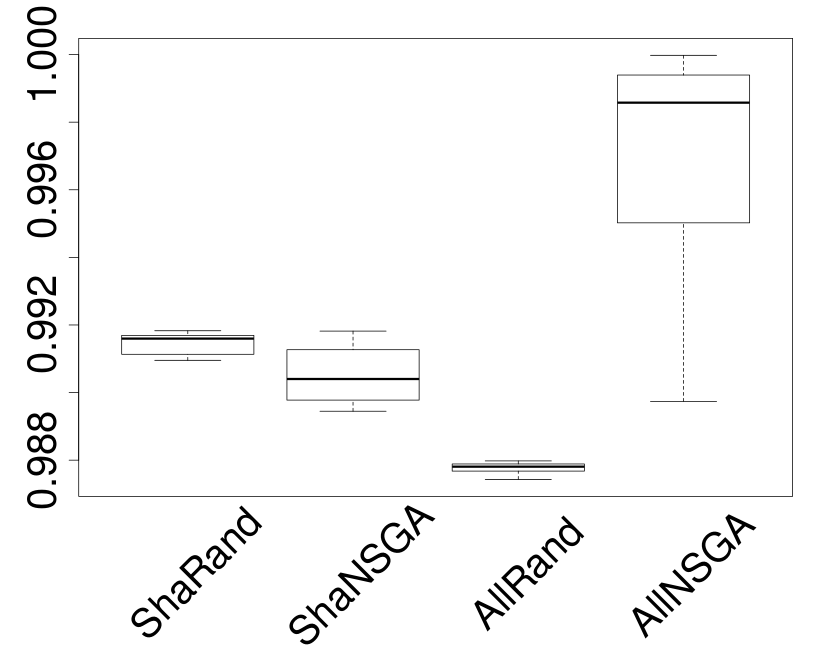
\includegraphics[width=0.22\textwidth]{espresso_hypervolume}
	}
	\subfigure[gawk]{
		\label{fig_hypervolume_gawk}
		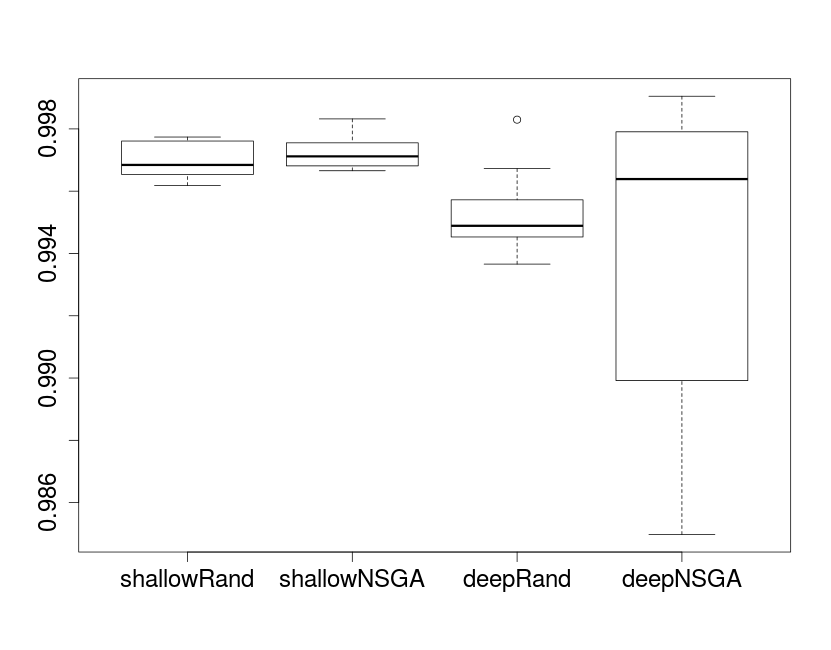
\includegraphics[width=0.22\textwidth]{gawk_hypervolume}
	}
	\subfigure[flex]{
		\label{fig_hypervolume_flex}
		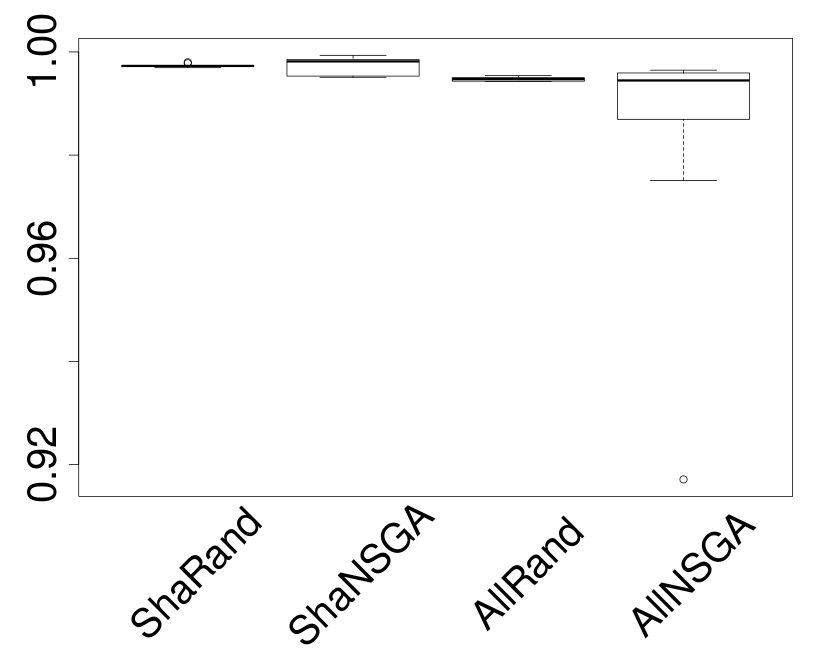
\includegraphics[width=0.22\textwidth]{flex_hypervolume}
	}
	\subfigure[sed]{
		\label{fig_hypervolume_sed}
		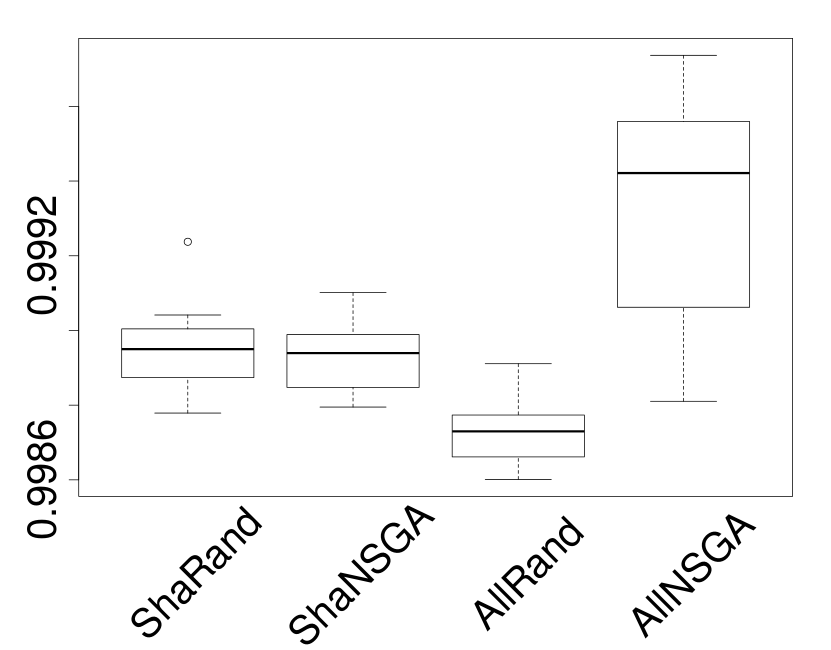
\includegraphics[width=0.22\textwidth]{sed_hypervolume}
	}
	\caption{Hypervolume indicator of Random, Shallow and Deep on all subjects. Bigger value is better.}\label{fig_hypervolume}
\end{figure}

\begin{figure}[htbp]
	\centering
	\subfigure[espresso]{
		\label{fig_contribution_espresso}
		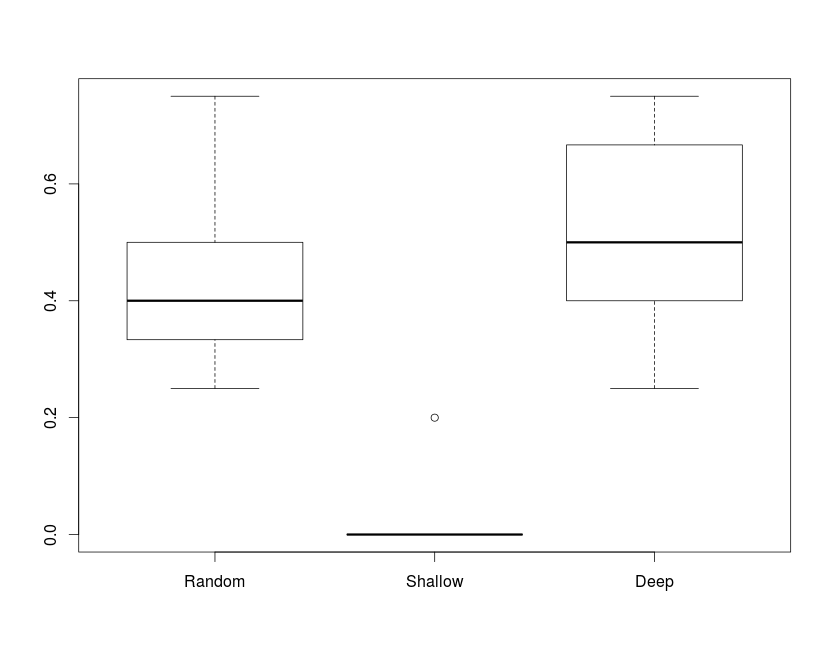
\includegraphics[width=0.22\textwidth]{espresso_contribution}
	}
	\subfigure[gawk]{
		\label{fig_contribution_gawk}
		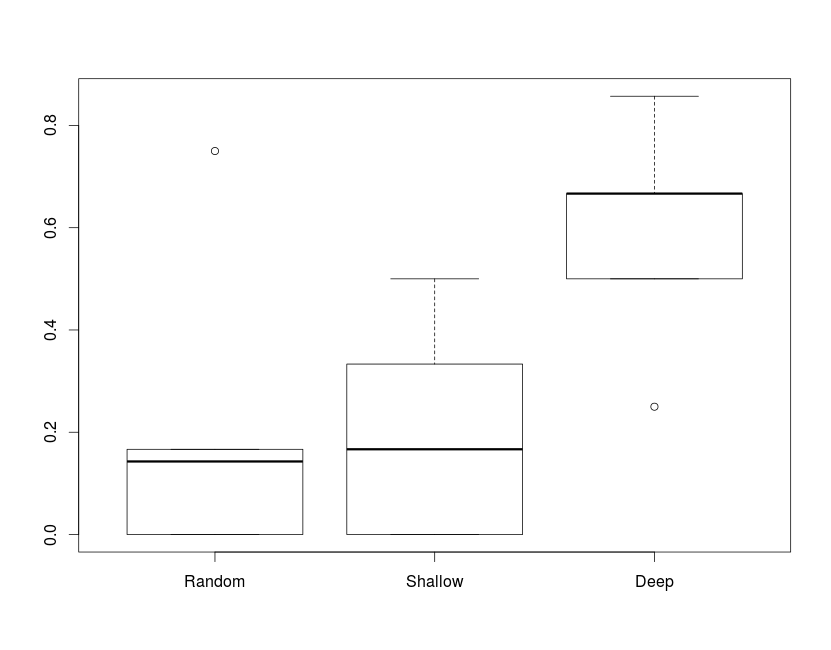
\includegraphics[width=0.22\textwidth]{gawk_contribution}
	}
	\subfigure[flex]{
		\label{fig_contribution_flex}
		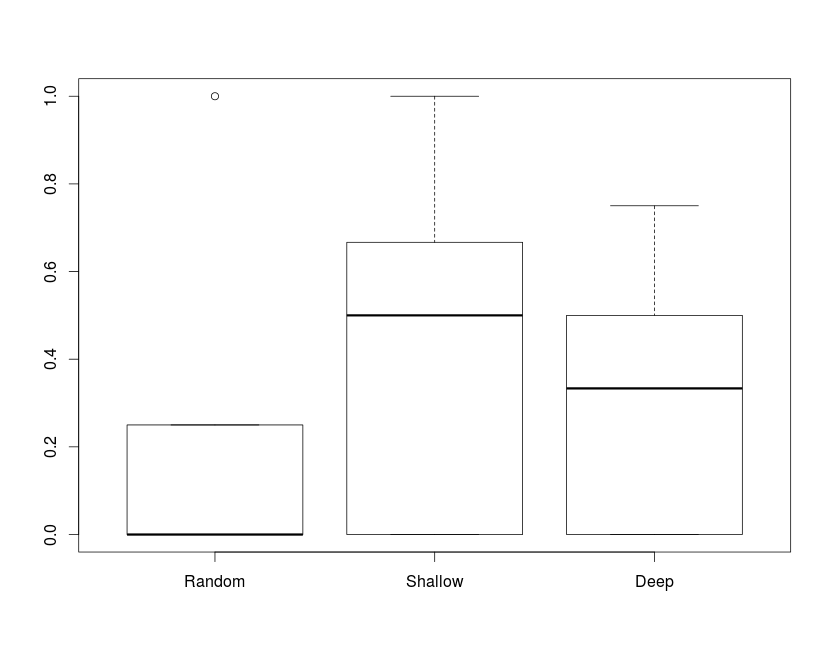
\includegraphics[width=0.22\textwidth]{flex_contribution}
	}
	\subfigure[sed]{
		\label{fig_contribution_sed}
		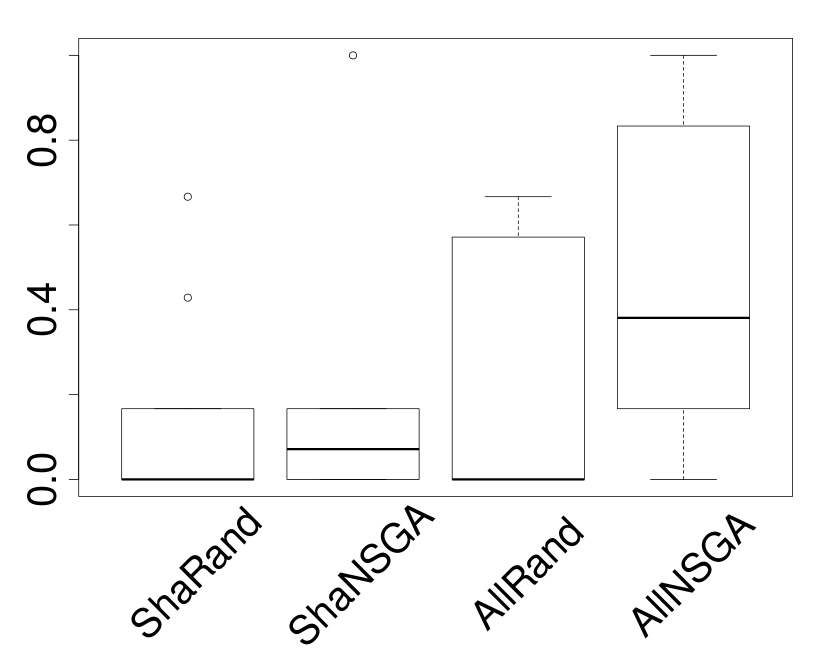
\includegraphics[width=0.22\textwidth]{sed_contribution}
	}
	\caption{Contribution indicator of Random, Shallow and Deep on all subjects. Bigger value is better.}\label{fig_contribution}
\end{figure}

\begin{figure}[htb]
	\centering
	\subfigure[espresso]{
		\label{fig_diversity_espresso}
		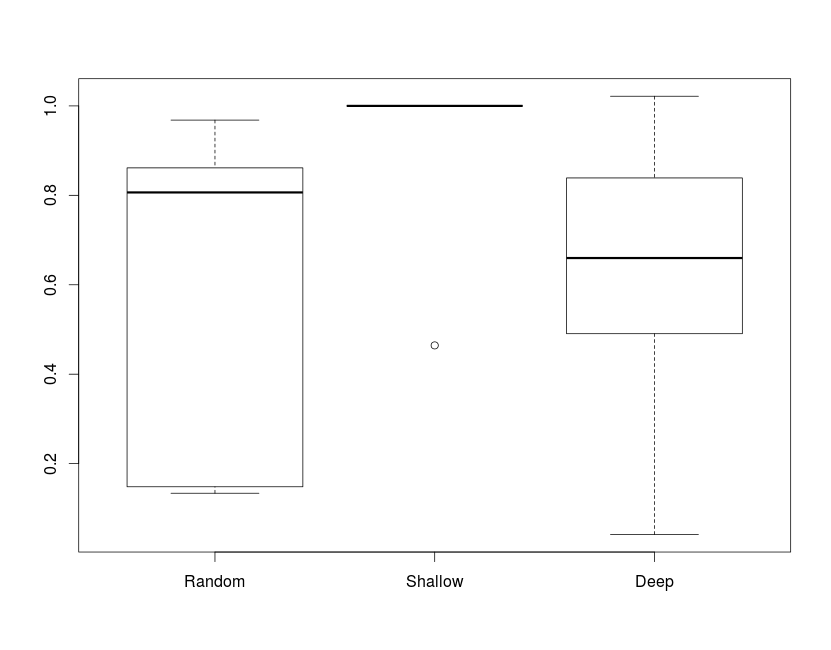
\includegraphics[width=0.22\textwidth]{espresso_diversity}
	}
	\subfigure[gawk]{
		\label{fig_diversity_gawk}
		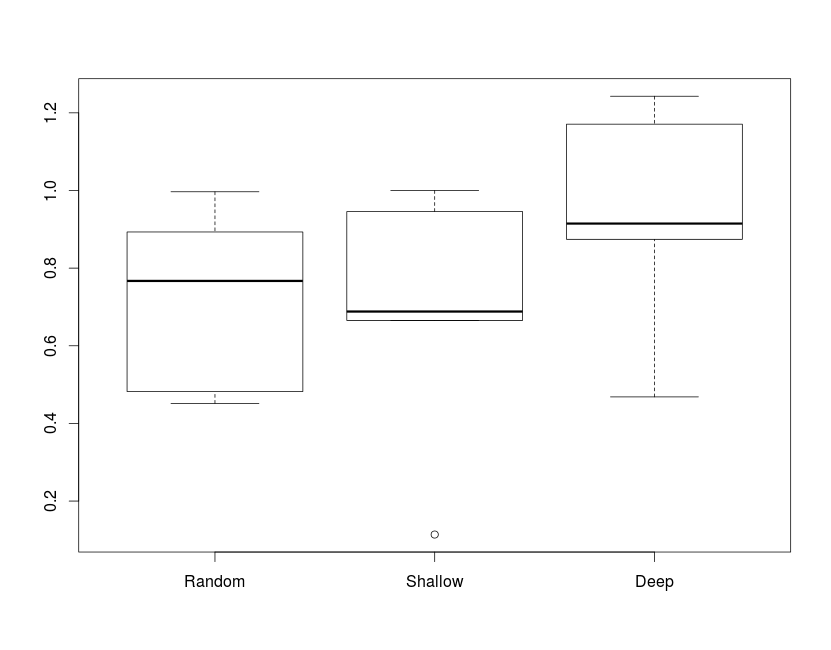
\includegraphics[width=0.22\textwidth]{gawk_diversity}
	}
	\subfigure[flex]{
		\label{fig_diversity_flex}
		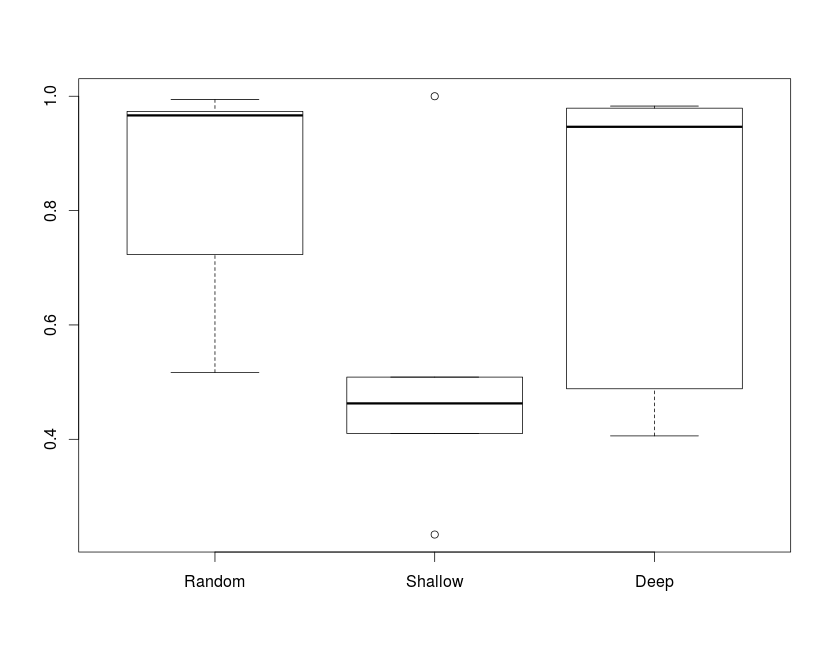
\includegraphics[width=0.22\textwidth]{flex_diversity}
	}
	\subfigure[sed]{
		\label{fig_diversity_sed}
		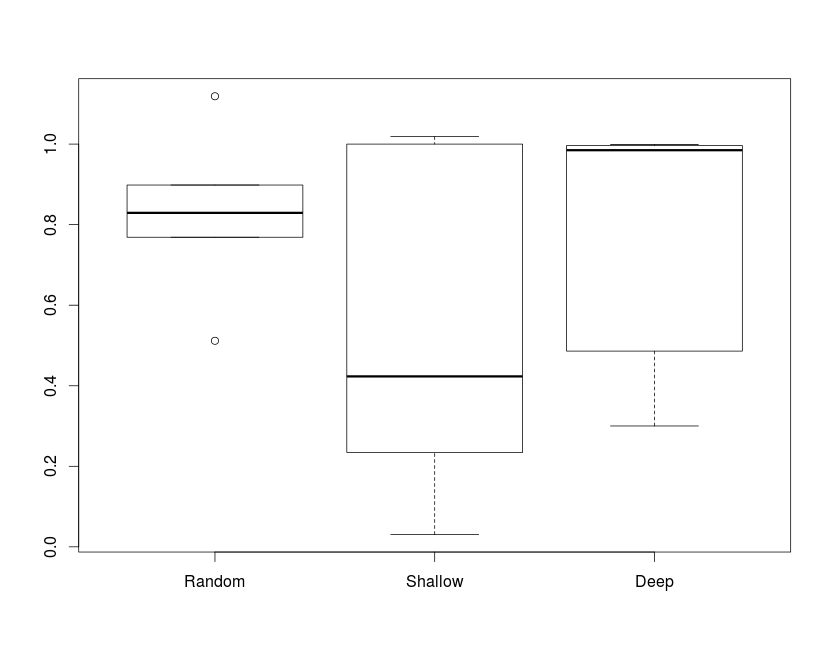
\includegraphics[width=0.22\textwidth]{sed_diversity}
	}
	\caption{Diversity indicator of Random, Shallow and Deep on all subjects. Smaller value is better.}\label{fig_diversity}
\end{figure}

\begin{figure}[htb]
	\centering
	\subfigure[espresso]{
		\label{fig_best_time_espresso}
		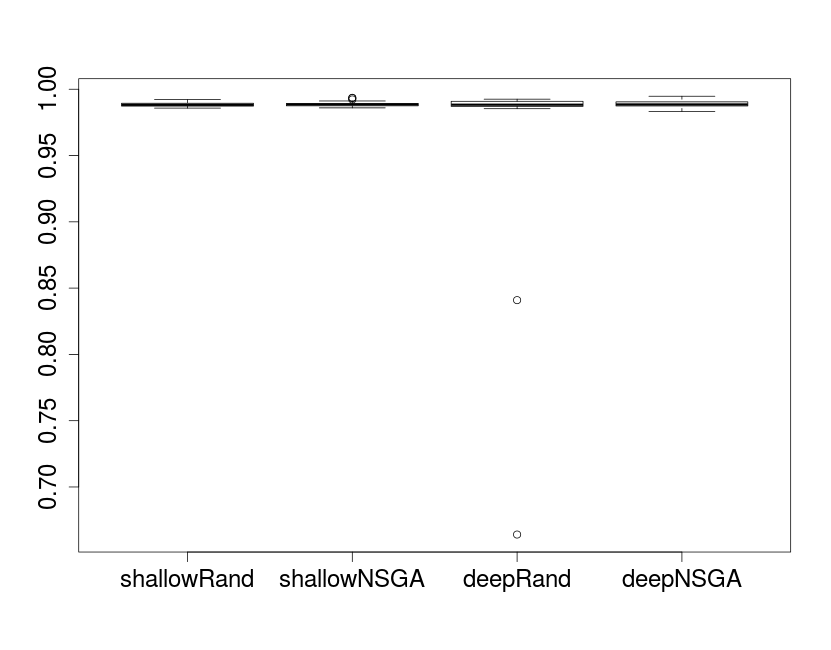
\includegraphics[width=0.22\textwidth]{espresso_best_time}
	}
	\subfigure[gawk]{
		\label{fig_best_time_gawk}
		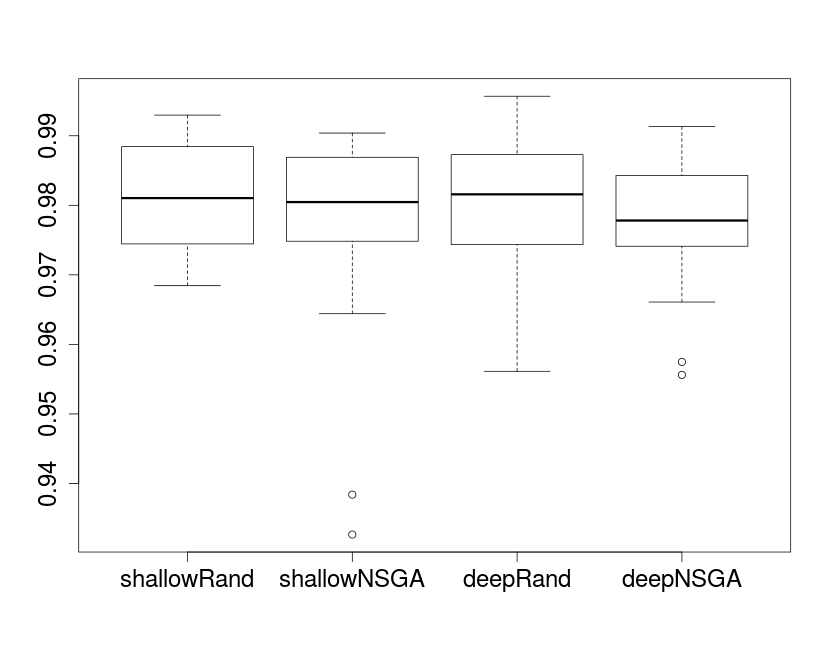
\includegraphics[width=0.22\textwidth]{gawk_best_time}
	}
	\subfigure[flex]{
		\label{fig_best_time_flex}
		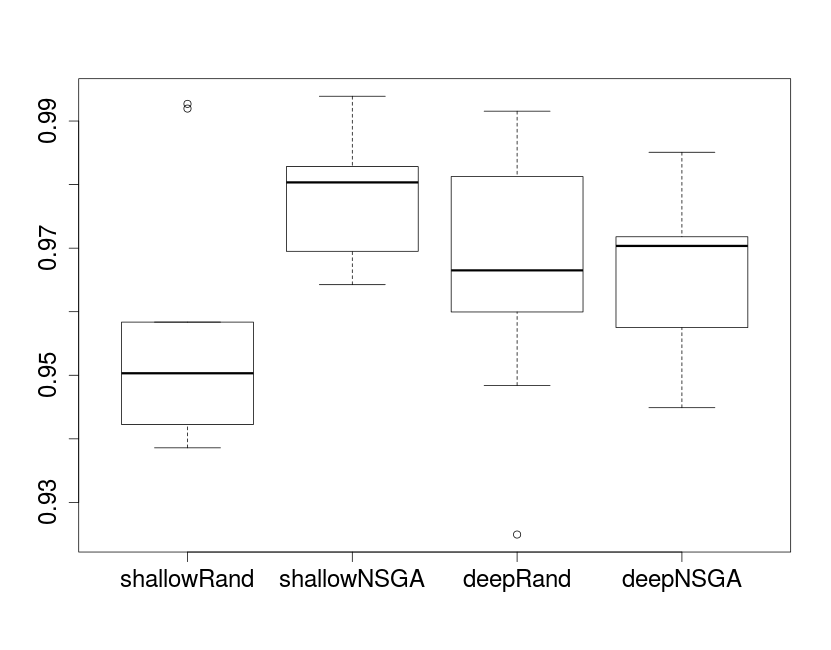
\includegraphics[width=0.22\textwidth]{flex_best_time}
	}
	\subfigure[sed]{
		\label{fig_best_time_sed}
		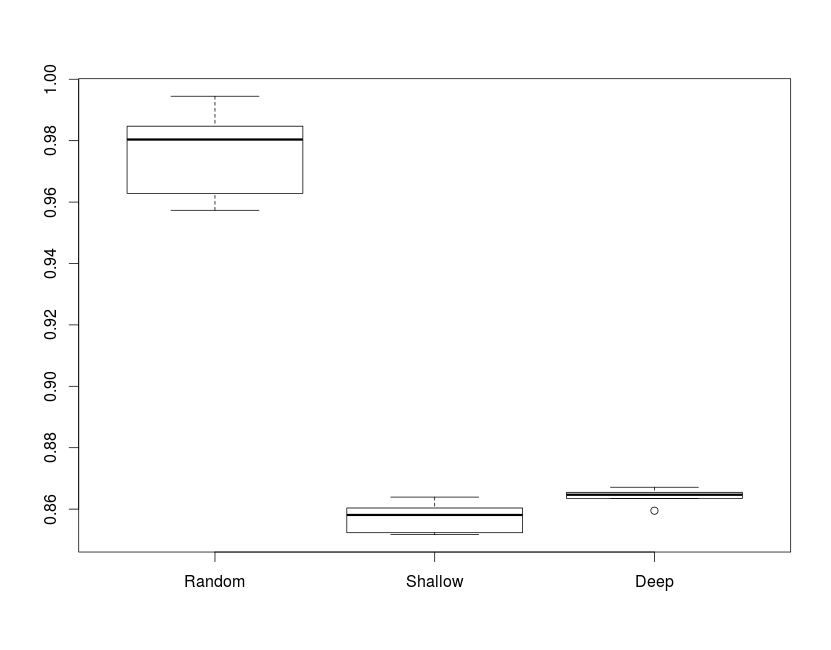
\includegraphics[width=0.22\textwidth]{sed_best_time}
	}
	\caption{The most time-saving performance found by each algorithm. Less is better.}\label{fig_best_time}
\end{figure}

\begin{figure}[htb]
	\centering
	\subfigure[espresso]{
		\label{fig_best_time_espresso}
		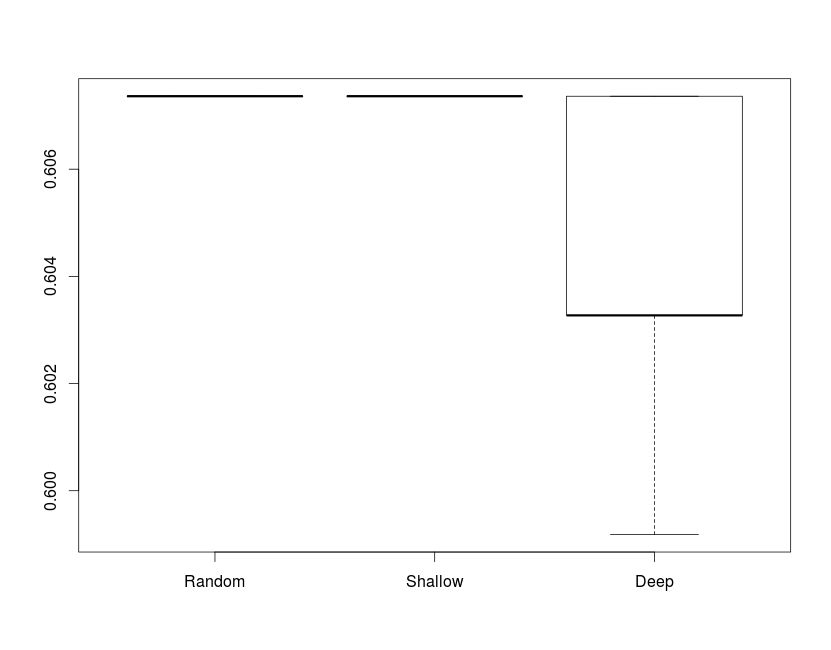
\includegraphics[width=0.22\textwidth]{espresso_best_memory}
	}
	\subfigure[gawk]{
		\label{fig_best_time_gawk}
		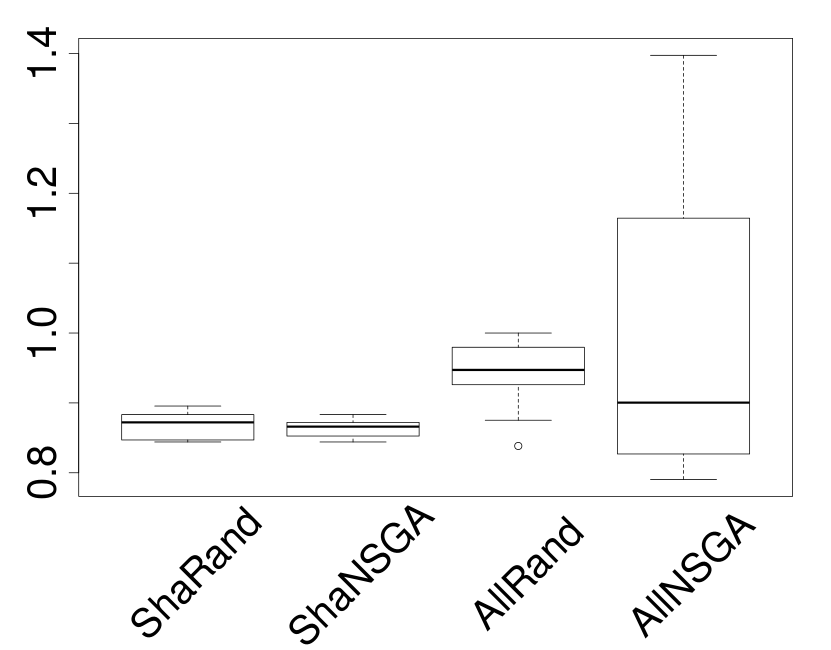
\includegraphics[width=0.22\textwidth]{gawk_best_memory}
	}
	\subfigure[flex]{
		\label{fig_best_time_flex}
		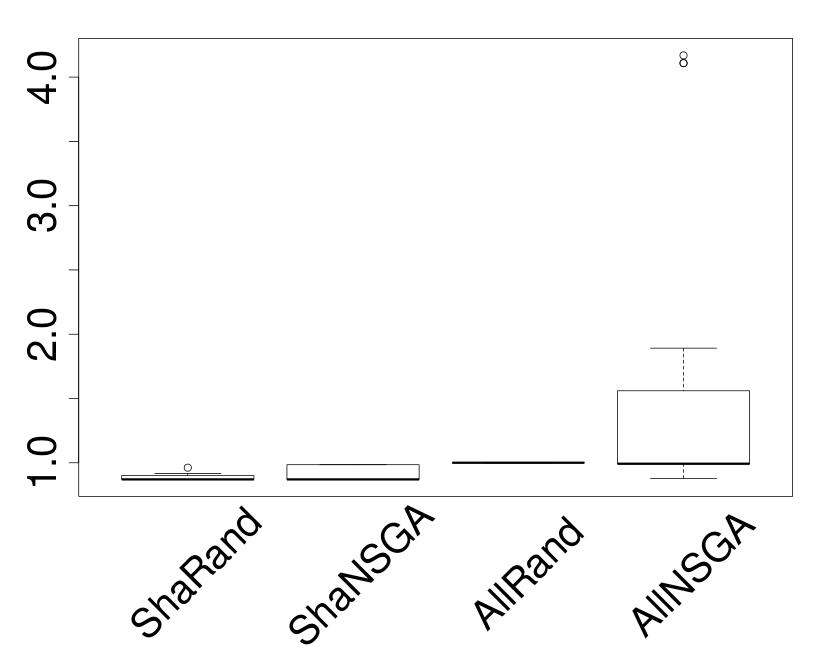
\includegraphics[width=0.22\textwidth]{flex_best_memory}
	}
	\subfigure[sed]{
		\label{fig_best_time_sed}
		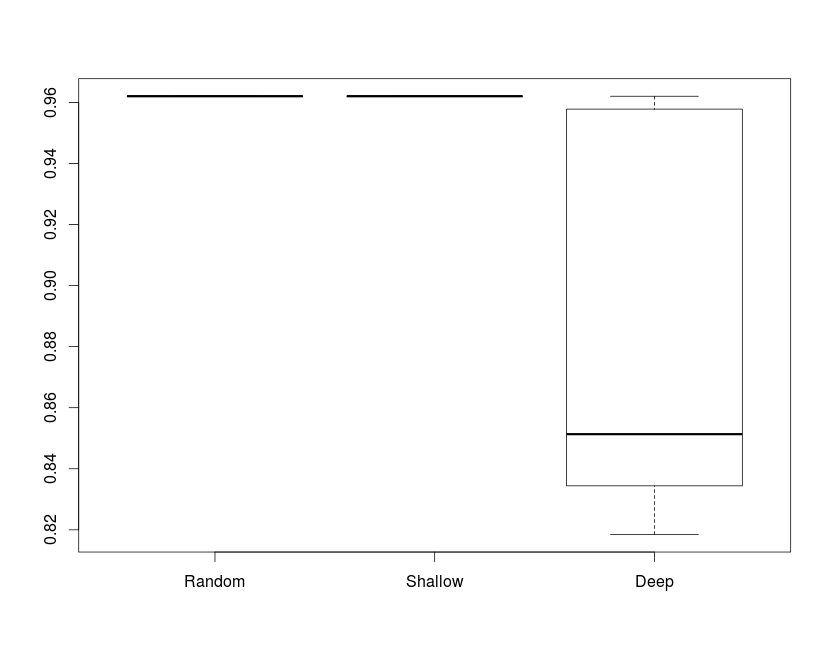
\includegraphics[width=0.22\textwidth]{sed_best_memory}
	}
	\caption{The most time-saving performance found by each algorithm. Less is better.}\label{fig_best_memory}
\end{figure}

To have a more quantative look at up to how much time and memory we can save from the original by our approach, we collect the best performance in terms of time and memory from all 30 runs for each subject-algorithm pair. The result is list in Table \ref{table_best_time_memory}. As clearly showed, Deep algorithm provides the possibility to further reduce the memory consumption.

% Please add the following required packages to your document preamble:
% \usepackage{multirow}
\begin{table*}[htbp]
\centering
\caption{Maximum reduction on time and memory for each algorithm and each subject}
\label{table_best_time_memory}
\begin{tabular}{|c|r|r|r|r|r|r|r|r|}
\hline
\multirow{2}{*}{\begin{tabular}[c]{@{}c@{}}Subject\\ Name\end{tabular}} & \multirow{2}{*}{\begin{tabular}[c]{@{}r@{}}Time\\ Original\end{tabular}} & \multicolumn{3}{r|}{Time Reduction} & \multirow{2}{*}{\begin{tabular}[c]{@{}r@{}}Memory Original\\ (Peak/Wasted)\end{tabular}} & \multicolumn{3}{r|}{Memory Waste Reduction} \\ \cline{3-5} \cline{7-9} 
                                                                        &                                                                          & Random     & Shallow    & Deep      &                                                                                          & Random       & Shallow       & Deep         \\ \hline
espresso                                                                & 4.75s                                                                    & 2.0\%      & 1.6\%      & 42.9\%    & 5152/978KB                                                                               & 39.3\%       & 39.3\%        & 40.1\%       \\ \hline
gawk                                                                    & 6.61s                                                                    & 3.3\%      & 2.8\%      & 2.6\%     & 29680/3552KB                                                                             & 15.1\%       & 15.1\%        & 16.8\%       \\ \hline
flex                                                                    & 0.13s                                                                    & 9.8\%      & 3.1\%      & 6.0\%     & 10816/525KB                                                                              & 13.0\%       & 13.0\%        & 13.0\%       \\ \hline
sed                                                                     & 0.25s                                                                    & 4.3\%      & 14.8\%     & 14.0\%    & 7048/948KB                                                                               & 3.8\%        & 3.8\%         & 18.2\%       \\ \hline
\end{tabular}
\end{table*}

To answer RQ3, we manually inspect the Deep Parameters exposed from each subject program and analyse why this parameter could infect the time/memory performance of a program. There are in total 23 distinct expressions from which Deep Parameters are exposed with respect to all four subjects. Among them, five expressions are found twice by Mutation-based sensitivity analysis on two different subjects, one is found three times and two are found on all four subjects. According to our knowledge to \emph{dlmalloc}, 12 out of all 23 distinct expressions make sense that they would affect the performance if their values are changed. Moreover, 7 out of 8 expressions that are found more than once are reasonable. Due to limit space, we can only explain why the two expressions found from all subjects can affect the performance in the rest of this section.

\begin{figure}[ht]
\begin{lstlisting}
1 static void* sys_alloc(mstate m,size_t nb) 
2 {
3 ...
4     /* Subtract out existing available top 
         space from MORECORE request. */
5     ssize = granularity_align(nb - m->topsize
         + SYS_ALLOC_PADDING+EXPOSE_4334);
6 ...
7     if (is_global(m))
8         init_top(m, (mchunkptr)tbase, tsize
              - TOP_FOOT_SIZE+EXPOSE_4425);
9 ...
8 }

\end{lstlisting}
\label{deep_parameter}
\caption{Deep Parameter Examples}
\end{figure}

The examples are shown in Figure \ref{deep_parameter}. Both of these two Deep Parameters are exposed from the function \emph{sys\_alloc()}, which manages most of the allocation from the system. The fist expression containing \emph{EXPOSE\_4334} is executed when the top chunk is not big enough to serve the memory requet and is about to be extended in system's dynamic memory, and the value of this expression decides how much memory should be get from the system this time. Smaller values tend to save memory, but may cause the program extend the top chunk more frequently, thus a waste of time. And how much memory should be get at this point may vary from applications to applications, so we expose a Deep Parameter from here so that we can control the size to be extended accordingly. The second example happens when initializing the heap. The value of the expression containing \emph{EXPOSE\_4425} is used to determine how much memory should be pre-allocated at the first time. For similar reason, bigger values tend to waste memory but save time.
